% LTeX: language=en-GB
%Author(s), Course variables
\newcommand{\titl}{02132 Assignment 2 report}
\newcommand{\subtitl}{Hardware implementation in Chisel\\of a small CPU running the image erosion}
\newcommand{\authone}{Mikkel Arn Andersen}
\newcommand{\SIDone}{s224187}
\newcommand{\authtwo}{Niclas Juul Schæffer}
\newcommand{\SIDtwo}{s224744}
\newcommand{\auththree}{Rasmus Kronborg Finnemann Wiuff}
\newcommand{\SIDthree}{s163977}
\newcommand{\lb}{\\}
%Basics
\documentclass[a4paper, english]{article}
\usepackage[utf8]{inputenc}
\usepackage[T1]{fontenc}
\usepackage[bitstream-charter]{mathdesign}
\usepackage{babel}
\usepackage[moderate, mathspacing=normal]{savetrees}
%Symbols and scientifics
\usepackage{bm}
\usepackage{physics}
\usepackage{mathtools}
\numberwithin{equation}{section}
\usepackage{siunitx}
\sisetup{
per-mode = power ,
round-mode = figures ,
round-precision = 3 ,
exponent-mode = input ,
output-decimal-marker = {.} ,
exponent-product = 	imes ,
uncertainty-mode = separate ,
range-phrase = - ,
range-units =  single ,
inter-unit-product = \ensuremath{{\cdot{}}} ,
quantity-product = \ ,
separate-uncertainty-units = single ,
}

%Appendix, TOC and Bibliography
\usepackage{appendix}
\renewcommand\appendixtocname{Appendix}
\usepackage[nottoc]{tocbibind}
\setcounter{tocdepth}{2}
\usepackage{lastpage}

%Figures
\usepackage[svgnames]{xcolor} % Required to specify font color
\usepackage{float}
\usepackage{graphicx}
\usepackage{subcaption}
\usepackage[format=plain,
    labelfont={bf,it,footnotesize},
    textfont={it,footnotesize}]{caption}
% \captionsetup[table]{name=Huskeord}
\captionsetup{font={stretch=0.9}}
\usepackage{wrapfig}
\usepackage[a4paper, centering, rmargin=2.5cm, tmargin=2.5cm, lmargin=2.5cm, bmargin=3.5cm]{geometry}
\usepackage{verbatim}
\usepackage[space]{grffile}
\usepackage[final]{pdfpages}
\usepackage{pdflscape}
\usepackage{multirow}
\usepackage{fontawesome}
\usepackage{tikz}
% \usetikzlibrary{external}
% \tikzexternalize[prefix=tikz/]
\usepackage{circuitikz}
\ctikzset{logic ports = ieee}
\usetikzlibrary{positioning}
\newcommand{\pin}[3]{\node[blue, font = \small, #2] at (#1) {#3};
                     \coordinate (#3) at (#1);}
\newcommand{\port}[4]{\node[circ, #2] (#1) {};
                     \node[#3] at (#1) {#4};}
%Header footer
\usepackage{fancyhdr}
\pagestyle{fancy}
\lhead{02132 Computer Systems \lb Assignment 1 \lb November \nth{12}}
\chead{
\includegraphics[width=.05\textwidth]{DTU}}
\rhead{\authone \ \textbf{\SIDone} \lb \authtwo \ \textbf{\SIDtwo} \lb \auththree \ \textbf{\SIDthree}}
\cfoot{Page \thepage\, of\, \pageref*{LastPage}}
\renewcommand{\headrulewidth}{0.4pt}
\renewcommand{\footrulewidth}{0.4pt}
\setlength{\headheight}{36.75034pt}

%Text tools
\usepackage{listings}
\usepackage{parcolumns}
\usepackage[super]{nth}
\usepackage[normalem]{ulem}
\usepackage{import}
\usepackage{url}
\usepackage{lipsum}
\usepackage{microtype}
\usepackage[pdfencoding=auto, psdextra]{hyperref}
\hypersetup{
    colorlinks   = true, %Colours links instead of ugly boxes
    urlcolor     = blue, %Colour for external hyperlinks
    linkcolor    = blue, %Colour of internal links
    citecolor   = red %Colour of citations
}
\usepackage[capitalise]{cleveref}
% \crefname{table}{Huskeord}{Huskeord}
\usepackage{enumitem}
\newlist{arrowlist}{itemize}{1}
\setlist[arrowlist]{label={\(\rightarrow\)}}
\usepackage{tabularray}
\UseTblrLibrary{booktabs}
\usepackage{todonotes}
\usepackage[square, longnamesfirst, numbers]{natbib}
\usepackage{empheq}
% \usepackage[newfloat, outputdir=/]{minted} % Overleaf minted buildpath fix
\usepackage[newfloat]{minted}
\setminted{fontsize=\small,
           linenos=true}
\usemintedstyle{tango}
\SetupFloatingEnvironment{listing}{listname=Listings}
\captionsetup[listing]{position=top, skip=-1pt}
\newcommand{\im}[3]{\inputminted[linenos=true, python3=true, firstline=#2, lastline=#3]{python}{#1}}
\newcommand{\java}[3]{\inputminted[linenos=true, firstline=#2, lastline=#3]{java}{#1}}
\usepackage{dirtree}

%Definitions and new commands
\newcommand{\degr}{^{\circ}}
\newcommand{\me}{\mathrm{e}}

%Title and sectioning
\def\Vhrulefill{\leavevmode\leaders\hrule height 0.7ex depth \dimexpr0.4pt-0.7ex\hfill\kern0pt}
\usepackage{titlesec}
\usepackage{titling}
\definecolor{DTUred}{cmyk}{0, .91, .72, .23}
\definecolor{FMNgrey}{cmyk}{.73,.43,.53,.38}
%Use letters insted of numbers in section numbering
% \renewcommand{\thesection}{\Alph{section}}
% \renewcommand{\thesubsection}{\Alph{subsection}}

\makeatletter
\newcommand{\github}[1]{%
   \href{#1}{\color{DTUred}\faGithub}%
}
\makeatother

%Algorithms and pseudocode
\newcounter{nalg}[section] % defines algorithm counter for chapter-level
\renewcommand{\thenalg}{\thesection .\arabic{nalg}} %defines appearance of the algorithm counter
\DeclareCaptionLabelFormat{algocaption}{Algoritme \thenalg} % defines a new caption label as Algorithm x.y

\lstnewenvironment{algorithm}[1][] %defines the algorithm listing environment
{
    \refstepcounter{nalg} %increments algorithm number
    \captionsetup{labelformat=algocaption,labelsep=colon} %defines the caption setup for: it ises label format as the declared caption label above and makes label and caption text to be separated by a ':'
    \lstset{ %this is the stype
        mathescape=true,
        frame=tB,
        numbers=left,
        numberstyle=\tiny,
        basicstyle=\scriptsize,
        keywordstyle=\color{black}\bfseries\em,
        keywords={,input, output, return, datatype, function, in, if, else, foreach, for, while, begin, end, do,} %add the keywords you want, or load a language as Rubens explains in his comment above.
        numbers=left,
        xleftmargin=.04\textwidth,
        columns=fullflexible,
        escapechar=\&,
        #1 % this is to add specific settings to an usage of this environment (for instnce, the caption and referable label)
    }
}
{}
\newcommand*{\runtimeAnalysis}[3]{\hfill\makebox[#3em][l]{\(#1\)}\hspace{5em}\makebox[#3em][l]{\(#2\)}}%

\begin{document}

\titleformat{\section}[block]
{\normalfont\Large\scshape\filright\color{DTUred}}{\fbox{\thesection}}{1em}{}

\titleformat{\subsection}
{\titlerule
    \vspace{.8ex}%
    \normalfont\scshape\color{FMNgrey}}
{\thesubsection.}{.5em}{}

\titleformat{\subsubsection}[wrap]
{\normalfont\fontseries{b}\selectfont\filright}
{\thesubsubsection.}{.5em}{}
\titlespacing{\subsubsection}
{12pc}{1.5ex plus .1ex minus .2ex}{1pc}

\title{\vspace{-40mm}\Huge\scshape\color{DTUred} \titl\lb\vspace{-4mm}\rule{4cm}{0.5mm}\lb\Large{\subtitl}}
\date{November \nth{12}}
\preauthor{\begin{center}
        \large \lineskip 0.5em%
        \begin{tabular}[t]{r}}
            \author{\textbf{Group: 22} \lb \lb \authone \ \textbf{\SIDone} \lb \authtwo \ \textbf{\SIDtwo} \lb \auththree \ \textbf{\SIDthree} \lb \href{https://github.com/rwiuff/02132Assignment2}{\color{DTUred}github.com/rwiuff/02132Assignment2} \github{https://github.com/rwiuff/02132Assignment2}}
            \postauthor{\end{tabular}\par\end{center}}
\maketitle

\pagenumbering{arabic}

\thispagestyle{empty}

\section{Work distribution}
\cref{tbl:ansvar} shows the work distribution for this project.
\begin{table}[H]
    \centering
    \caption{Work distribution on the project}\label{tbl:ansvar}
    \begin{tabular}{lll}
        \toprule
        Name                 & Development tasks                                         & Report tasks                                \\
        \midrule
        Mikkel Arn Andersen  & Assembler: Memory test, arithmetic test, jump test.       & \cref{sec:test}                             \\
                             & Implementation evaluation.                                &                                             \\
        \midrule
        Niclas Juul Schæffer & CPU Block design, ALU implementation,                     & \cref{sec:implement}                        \\
                             & CPUTop implementation, Register File implementation,      &                                             \\
                             & Chisel testers.                                           &                                             \\
        \midrule
        Rasmus Wiuff         & ISA, assembler compilation, machine instruction encoding, & \cref{sec:isa,sec:compileandencode,sec:CPU} \\
                             & CPU Block design, Program Counter implementation,         &                                             \\
                             & Control Unit implementation.                              &                                             \\
        \bottomrule
    \end{tabular}
\end{table}
\section{Design}
The project requirements were open to broad interpretation, so first step of the design was to put on restrictions. The following was stipulated:
\begin{enumerate}
    \item All blocks in the assignment would be laid out as described in the material.
    \item The architecture would be 32-bit.
    \item The instruction set architecture should be as simple as possible, but still versatile.
\end{enumerate}
The next step was designing the instruction set architecture and the encoding scheme.
\subsection{ISA and encoding scheme}\label{sec:isa}
The instruction set needs to contain basic arithmetic operations as well as logical ones for computations. Instructions are also needed for creating variables in the registers as well as reading and writing data between registers and memory. A branch (or in this project jump) instruction is needed to navigate between instruction lines as well as at least one conditional branch instruction. Lastly the program needs to terminate. The chosen instructions are listed in \cref{tbl:ISA}.
\begin{table}
    \centering
    \caption{Instruction set architecture used in the assignment}\label{tbl:ISA}
    \begin{tabular}{lll}
        \toprule
        \textbf{Instruction}     & \textbf{Syntax}          & \textbf{Meaning}                 \\
        \midrule
        \multicolumn{3}{c}{Arithmetic instructions}                                            \\
        \midrule
        Addition                 & \texttt{ADD Rx, Ry, Rz;} & \texttt{Rx = Ry + Rz}            \\
        Subtraction              & \texttt{SUB Rx, Ry, Rz;} & \texttt{Rx = Ry - Rz}            \\
        Immediate addition       & \texttt{ADDI Rx, Ry, z;} & \texttt{Rx = Ry + z}             \\
        Immediate subtraction    & \texttt{SUBI Rx, Ry, z;} & \texttt{Rx = Ry - z}             \\
        Immediate multiplication & \texttt{MULT Rx, Ry, z;} & \texttt{Rx = Ry \(\cdot\) z}     \\
        Increment                & \texttt{INC, Rx}         & \texttt{Rx = Rx + 1}             \\
        \midrule
        \multicolumn{3}{c}{Logic instructions}                                                 \\
        \midrule
        Bitwise OR               & \texttt{OR Rx, Ry, Rz;}  & \texttt{Rx = Ry \(\vert\) Rz}    \\
        Bitwise AND              & \texttt{AND Rx, Ry, Rz;} & \texttt{Rx = Ry \(\&\) Rz}       \\
        \midrule
        \multicolumn{3}{c}{Memory instructions}                                                \\
        \midrule
        Load immediate           & \texttt{LOADI Rx, y;}    & \texttt{Rx = y}                  \\
        Load data                & \texttt{LOAD Rx, Ry;}    & \texttt{Rx = memory(Ry)}         \\
        Store data               & \texttt{STORE Rx, Ry;}   & \texttt{memory(Ry) = Rx}         \\
        \midrule
        \multicolumn{3}{c}{Control and flow instructions}                                      \\
        \midrule
        Jump                     & \texttt{JMP x}           & \texttt{GOTO INST x}             \\
        Jump if equal            & \texttt{JEQ Rx, Ry, z;}  & \texttt{if(Rx > Ry) GOTO INST z} \\
        END                      & \texttt{END;}            & \texttt{Terminate}               \\
        \bottomrule
    \end{tabular}
\end{table}
A total of 14 instructions are settled upon. This requires \(\lceil \log_2{14} \rceil = 4\) bits for the opcode part of the instruction. As defined in the assignment, the memory block has an input of 16 bits. This, with the 4 opcode bits, leaves 12 bits for register addresses. Consequently, this limits the chip to 16 registers. The instruction scheme is shown in \cref{fig:inst}.
\begin{figure}
    \centering
    \centering
    \caption{Instruction layout. Ra and Rb are operands, Rd is the destination register. Remaining bits are used for either memory address or immediate value.}\label{fig:inst}
    \resizebox{\textwidth}{!}{%
        \begin{tikzpicture}
            \draw[black, very thick] (0,0) rectangle (32,2); % INST box
            \draw[fill=green!20] (0,0) rectangle (4,2); % OPCODE section
            \draw[fill=red!20] (4,0) rectangle (8,2); % Reg section
            \draw[fill=blue!20] (8,0) rectangle (12,2); % Reg section
            \draw[fill=yellow!20] (12,0) rectangle (16,2); % Reg section
            \draw[fill=cyan!20] (16,0) rectangle (32,2); % Value section
            \node[align=center] (opcode) at (2,1) {\Large OPCODE (4 bits) \\ \Large 31 \(\cdots\) 28};
            \node[align=center] (rd) at (6,1) {\Large Rd (4 bits) \\ \Large 27 \(\cdots\) 24};
            \node[align=center] (r1) at (10,1) {\Large Ra (4 bits) \\ \Large 23 \(\cdots\) 20};
            \node[align=center] (r2) at (14,1) {\Large Rb (4 bits) \\ \Large 19 \(\cdots\) 16};
            \node[align=center] (val) at (24,1) {\Large Value/address (16 bit) \\ \Large 15 \(\cdots\) 0};
        \end{tikzpicture}
    }%
\end{figure}
\cref{tbl:encex} shows how each instruction can be encoded into 32 bits. Notice how, when writing or reading to/from memory, \texttt{Rb} points to the register with the memory address. This makes the wiring in the CPU block easier, as a wire from the \(b\) output of the register file can be connected directly to the address input port in the data memory.
\begin{table}
    \centering
    \caption{Encoding instructions under the instruction set and encoding scheme}\label{tbl:encex}
    \begin{tabular}{llllll}
        \toprule
        \textbf{Instruction}     & OPCODE        & Rd            & Ra            & Rb            & Value/address                \\
        \midrule
        \texttt{ADD R1, R2, R3;} & \texttt{0001} & \texttt{0001} & \texttt{0010} & \texttt{0011} & \texttt{0000 0000 0000 0000} \\
        \texttt{SUB R1, R2, R3;} & \texttt{0010} & \texttt{0001} & \texttt{0010} & \texttt{0011} & \texttt{0000 0000 0000 0000} \\
        \texttt{ADDI R1, R2, 1;} & \texttt{0011} & \texttt{0001} & \texttt{0010} & \texttt{0000} & \texttt{0000 0000 0000 0001} \\
        \texttt{SUBI R1, R2, 1;} & \texttt{0100} & \texttt{0001} & \texttt{0010} & \texttt{0000} & \texttt{0000 0000 0000 0001} \\
        \texttt{MULT R1, R2, 1;} & \texttt{0101} & \texttt{0001} & \texttt{0010} & \texttt{0000} & \texttt{0000 0000 0000 0001} \\
        \texttt{OR R1, R2, R3;}  & \texttt{0110} & \texttt{0001} & \texttt{0010} & \texttt{0011} & \texttt{0000 0000 0000 0000} \\
        \texttt{AND R1, R2, R3;} & \texttt{0111} & \texttt{0001} & \texttt{0010} & \texttt{0011} & \texttt{0000 0000 0000 0000} \\
        \texttt{LOADI R1, 1;}    & \texttt{1000} & \texttt{0001} & \texttt{0000} & \texttt{0000} & \texttt{0000 0000 0000 0001} \\
        \texttt{LOAD R1, R2;}    & \texttt{1001} & \texttt{0001} & \texttt{0000} & \texttt{0010} & \texttt{0000 0000 0000 0000} \\
        \texttt{STORE R1, R2;}   & \texttt{1010} & \texttt{0000} & \texttt{0001} & \texttt{0010} & \texttt{0000 0000 0000 0000} \\
        \texttt{INC R1;}         & \texttt{1011} & \texttt{0001} & \texttt{0001} & \texttt{0000} & \texttt{0000 0000 0000 0000} \\
        \texttt{JMP 1;}          & \texttt{1100} & \texttt{0000} & \texttt{0000} & \texttt{0000} & \texttt{0000 0000 0000 0001} \\
        \texttt{JEQ R1, R2, 1;}  & \texttt{1101} & \texttt{0000} & \texttt{0001} & \texttt{0010} & \texttt{0000 0000 0000 0001} \\
        \texttt{END;}            & \texttt{1111} & \texttt{0000} & \texttt{0000} & \texttt{0000} & \texttt{0000 0000 0000 0000} \\
        \bottomrule
    \end{tabular}
\end{table}
\subsection{Compile and encode}\label{sec:compileandencode}
\subsubsection{Compiled to assembler}
In this project the provided algorithm is used. It is compiled by hand to assembler using the defined instruction set in \cref{tbl:ISA}. The program does the following:
\begin{itemize}
    \item Lines 0-4 set initial values.
    \item Lines 5-6 is the for loop conditional checks.
    \item Lines 7-9 contains the address for the pixel at \(x + y \times 20\).
    \item Lines 10-13 checks for image border case.
    \item Lines 14-17 checks the inner pixel.
    \item Lines 18-37 calculates the addresses for pixels at \(x - 1, x + 1, y - 1, y + 1\) and these pixels are loaded and compared with logic AND. The result is the compared to 0.
    \item Lines 38-39 is the branch if an output pixel is set to 255.
    \item Lines 40-41 is the branch if an output pixel is set to 0.
    \item Lines 42-43 increments \(y\) and jumps to the nested loop conditional check.
    \item Lines 44-46 increments \(x\), sets \(y\) to zero and jumps to the main loop conditional check.
    \item Line 47 terminates the program.
\end{itemize}
The registers are utilised in the following way:
\begin{itemize}
    \item R0 and R1 contains the current \(x\) and \(y\) counter.
    \item R2 contains the picture width in pixels.
    \item R3 and R4 hold the values 0 and 255 for conditional comparison and for writing either black or white pixels to the output image addresses.
    \item R5 holds the output image address for the current pixel.
    \item R6 to R15 are used for storage during calculations.
\end{itemize}
\begin{figure}
    \captionof{listing}{The program compiled to assembly}\label{lst:ass}
    \begin{minipage}{0.49\textwidth}
        \vspace{1.5em}
        \centering
        \begin{minted}[linenos = false]{mips}
        # Initial values
00. LOADI R0, 0;      # x counter
01. LOADI R1, 0;      # y counter
02. LOADI R2, 19;     # Pixel limit
03. LOADI R3, 0;      # Zero value
04. LOADI R4, 255;    # 255 value
        # For loop conditions
05. JEQ R0, R2, 47;   # Check x, GOTO END
06. JEQ R1, R2, 44;   # Check y, GOTO INC X
        # Output image address
07. MULT R5, R1, 20;  # y * 20
08. ADD R6, R0, R5;   # x + y * 20
09. ADDI R5, R6, 400; # Out image address
        # Process border pixel
10. JEQ R0, R3, 40;   # If x or y = 0
11. JEQ R1, R3, 40;   #
12. JEQ R0, R4, 40;   # If x or y = 19
13. JEQ R1, R4, 40;   # GOTO erosion
        # Process inner pixel
14. MULT R6, R1, 20;  # y * 20
15. ADD R7, R0, R6;   # x + y * 20
16. LOAD R8, R7;      # Get input pixel
17. JEQ R8, R3, 40;   # If 0, GOTO erosion
        # Process outer pixels
18. SUBI R12, R0, 1;  # x - 1
19. ADDI R13, R0, 1;  # x + 1
20. SUBI R14, R1, 1;  # y - 1
21. ADDI R15, R1, 1;  # y + 1
22. MULT R6, R1, 20;  # y * 20
23. ADD R7, R6, R12;  # (x - 1) + y * 20
    \end{minted}
    \end{minipage}
    \begin{minipage}{0.49\textwidth}
        \vspace{.5em}
        \centering
        \begin{minted}[linenos = false]{mips}
24. LOAD R8, R7;      # Save pixel in R8
25. MULT R6, R1, 20;  # y * 20
26. ADD R7, R6, R13;  # (x + 1) + y * 20
27. LOAD R9, R7;      # Save pixel in R9
28. AND R10, R8, R9;  # AND R8 and R9, save to R10
29. MULT R6, R14, 20; # (y - 1) * 20
30. ADD R7, R6, R0;   # x + (y - 1) * 20
31. LOAD R8, R7;      # Save pixel in R8
32. AND R9, R8, R10;  # AND R8 and R10, save to R9
33. MULT R6, R15, 20; # (y + 1) * 20
34. ADD R7, R6, R0;   # x + (y + 1) * 20
35. LOAD R10, R7;     # Save pixel in R10
36. AND R8, R9, R10;  # AND R9 and R10, save to R8
37. JEQ R8, R3, 40;   # If = 0 GOTO Erosion
            # No erosion
38. STORE R4, R5;     # Set pixel to 255
39. JMP 42;           # GOTO increment y
            # Erosion
40. STORE R3, R5;     # Set Pixel to zero
41. JMP 42;           # GOTO increment y
            # Increment y
42. INC R1;           # Increment y
43. JMP 6;            # Continue nested loop
            # Increment x
44. INC R0;           # Increment x
45. LOADI R1, 0;      # Zerorise y
46. JMP 5;            # Continue main loop
            # Terminate program
47. END;              # Terminate program
     \end{minted}
    \end{minipage}
\end{figure}
\subsubsection{Encoding the program}
\cref{lst:ass} is encoded to machine instructions using the instruction scheme in \cref{tbl:encex}. \cref{lst:machine} shows the encoded program.
\begin{figure}
    \captionof{listing}{The encoded program}\label{lst:machine}
    \begin{minipage}{0.49\textwidth}
        \vspace{1.5em}
        \centering
        \begin{minted}[linenos = false]{mips}
    OP   Rd   Ra   Rb   Value/address
00. 1000 0000 0000 0000 0000000000000000
01. 1000 0001 0000 0000 0000000000000000
02. 1000 0010 0000 0000 0000000000010011
03. 1000 0011 0000 0000 0000000000000000
04. 1000 0100 0000 0000 0000000011111111
05. 1101 0000 0000 0010 0000000000101111
06. 1101 0000 0001 0010 0000000000101100
07. 0101 0101 0001 0000 0000000000010100
08. 0001 0110 0000 0101 0000000000000000
09. 0011 0101 0110 0000 0000000110010000
10. 1101 0000 0000 0011 0000000000101000
11. 1101 0000 0001 0011 0000000000101000
12. 1101 0000 0000 0100 0000000000101000
13. 1101 0000 0001 0100 0000000000101000
14. 0101 0110 0001 0000 0000000000010100
15. 0001 0111 0000 0110 0000000000000000
16. 1001 1000 0000 0111 0000000000000000
17. 1101 0000 1000 0011 0000000000101000
18. 0100 1100 0000 0000 0000000000000001
19. 0011 1101 0000 0000 0000000000000001
20. 0100 1110 0001 0000 0000000000000001
21. 0011 1111 0001 0000 0000000000000001
22. 0101 0110 0001 0000 0000000000010100
23. 0001 0111 0110 1100 0000000000000000
    \end{minted}
    \end{minipage}
    \begin{minipage}{0.49\textwidth}
        \vspace{1.5em}
        \centering
        \begin{minted}[linenos = false]{mips}
    OP   Rd   Ra   Rb   Value/address
24. 1001 1000 0000 0111 0000000000000000
25. 0101 0110 0001 0000 0000000000010100
26. 0001 0111 0110 1101 0000000000000000
27. 1001 1001 0000 0111 0000000000000000
28. 0111 1010 1000 1001 0000000000000000
29. 0101 0110 1110 0000 0000000000010100
30. 0001 0111 0110 0000 0000000000000000
31. 1001 1000 0000 0111 0000000000000000
32. 0111 1001 1000 1010 0000000000000000
33. 0101 0110 1111 0000 0000000000010100
34. 0001 0111 0110 0000 0000000000000000
35. 1001 1010 0000 0111 0000000000000000
36. 0111 1000 1001 1010 0000000000000000
37. 1101 0000 1000 0011 0000000000101000
38. 1010 0000 0100 0101 0000000000000000
39. 1100 0000 0000 0000 0000000000101010
40. 1010 0000 0011 0101 0000000000000000
41. 1100 0000 0000 0000 0000000000101010
42. 1011 0001 0001 0000 0000000000000000
43. 1100 0000 0000 0000 0000000000000110
44. 1011 0000 0000 0000 0000000000000000
45. 1000 0001 0000 0000 0000000000000000
46. 1100 0000 0000 0000 0000000000000101
47. 1111 0000 0000 0000 0000000000000000
     \end{minted}
    \end{minipage}
\end{figure}
\subsection{CPU block}\label{sec:CPU}
The CPU block is shown in \cref{fig:cpu}. Blue wires are control bits from the \texttt{ControlUnit}. Along with \cref{fig:cpu} this section will explain the connectivity from \texttt{ProgramCounter}(\texttt{PC}) to \texttt{RegisterFile} and \texttt{ControlUnit}. With these anchor points the rest is laid out.
\subsubsection{ProgramCounter and RegisterFile}
The \texttt{run} port drives the \texttt{PC}. \texttt{PC} in turn gives a 16-bit address to the \texttt{ProgramMemory}, which in turn outputs a 32-bit instruction. The instruction is split according to the instruction scheme. \texttt{Rd} connects to \texttt{writeSel} on the \texttt{RegisterFile}, \texttt{Ra} to \texttt{aSel} and \texttt{Rb} to \texttt{bSel}. The \texttt{Value/address} goes to the \texttt{PC} in case a jump is performed, and to a mux leading to the \texttt{ALU} in case an immediate value is used as a second operand. The \texttt{Extender} pads the 16-bit value to fit the 32-bit input in the mux. The \texttt{RegisterFile} outputs are connected to \texttt{DataMemory} with \texttt{a} to \texttt{dataWrite} and \texttt{b} to \texttt{address}.
\subsubsection{ControlUnit}
The last instruction piece contains \texttt{opcode} which goes into the \texttt{ControlUnit}. From here Driving bits are wired to various multiplexers and components. \texttt{writeToRegister} drives the \texttt{writeEnable} port and is on if data is to be saved in the \texttt{RegisterFile}. \texttt{writeToMemory} drives the \texttt{writeEnable} port and is on if data is to be saved in the \texttt{DataMemory}. \texttt{stop} goes to the \texttt{PC} and \texttt{done} output port and tells the system to terminate. \texttt{immediateJump} and \texttt{jump}, together with the first bit of the \texttt{ALU} result drives the \texttt{jump} port on the \texttt{PC}, according to \cref{tbl:jmpbits}.
\begin{table}[H]
    \centering
    \caption{ControlUnit jump bits}\label{tbl:jmpbits}
    \begin{tabular}{llll}
        \toprule
        \texttt{jump} & \texttt{immediateJump} & \texttt{alu.result} & \texttt{ProgramCounter.jump} \\
        \midrule
        \texttt{0}    & \texttt{0}             & \texttt{X}          & \texttt{0}                   \\
        \texttt{1}    & \texttt{0}             & \texttt{0}          & \texttt{0}                   \\
        \texttt{1}    & \texttt{0}             & \texttt{1}          & \texttt{1}                   \\
        \texttt{1}    & \texttt{1}             & \texttt{X}          & \texttt{1}                   \\
        \bottomrule
    \end{tabular}
\end{table}

\texttt{aluFunc} tells the \texttt{ALU} which operation to be performed. \texttt{immediateOperand} connects the \texttt{op2} input on the \texttt{ALU} with either the padded \texttt{Value/address} instruction or \texttt{b} port on \texttt{RegisterFile}.\newline
\texttt{immediateLoad} either connects the \texttt{ALU} \texttt{result} port or the \texttt{Value/address} instruction to the next mux, which is driven by \texttt{loadFromMemory}. Here either \texttt{result,Value/address} or \texttt{dataRead} on \texttt{DataMemory} is connected to \texttt{writeData} on \texttt{RegisterFile}.\newline
The opcode and corresponding control signals are shown in \cref{tbl:cu}.
\begin{table}[H]
    \centering
    \caption{ControlUnit control bits}\label{tbl:cu}
    \resizebox{\textwidth}{!}{
        \begin{tabular}{lllllllllllllll}
            \toprule
            \texttt{instruction}      & \texttt{ADD}  & \texttt{SUB}  & \texttt{ADDI} & \texttt{SUBI} & \texttt{MULT} & \texttt{OR}   & \texttt{AND}  & \texttt{LOADI} & \texttt{LOAD} & \texttt{STORE} & \texttt{INC}  & \texttt{JMP}  & \texttt{JEQ}  & \texttt{END}  \\
            \texttt{opcode}           & \texttt{0001} & \texttt{0010} & \texttt{0011} & \texttt{0100} & \texttt{0101} & \texttt{0110} & \texttt{0111} & \texttt{1000}  & \texttt{1001} & \texttt{1010}  & \texttt{1011} & \texttt{1100} & \texttt{1101} & \texttt{1111} \\
            \midrule
            \texttt{writeToRegister}  & \texttt{1}    & \texttt{1}    & \texttt{1}    & \texttt{1}    & \texttt{1}    & \texttt{1}    & \texttt{1}    & \texttt{1}     & \texttt{1}    & \texttt{0}     & \texttt{1}    & \texttt{0}    & \texttt{0}    & \texttt{0}    \\
            \texttt{stop}             & \texttt{0}    & \texttt{0}    & \texttt{0}    & \texttt{0}    & \texttt{0}    & \texttt{0}    & \texttt{0}    & \texttt{0}     & \texttt{0}    & \texttt{0}     & \texttt{0}    & \texttt{0}    & \texttt{0}    & \texttt{1}    \\
            \texttt{immediateJump}    & \texttt{0}    & \texttt{0}    & \texttt{0}    & \texttt{0}    & \texttt{0}    & \texttt{0}    & \texttt{0}    & \texttt{0}     & \texttt{0}    & \texttt{0}     & \texttt{0}    & \texttt{1}    & \texttt{0}    & \texttt{0}    \\
            \texttt{jump}             & \texttt{0}    & \texttt{0}    & \texttt{0}    & \texttt{0}    & \texttt{0}    & \texttt{0}    & \texttt{0}    & \texttt{0}     & \texttt{0}    & \texttt{0}     & \texttt{0}    & \texttt{1}    & \texttt{1}    & \texttt{0}    \\
            \texttt{aluFunc}          & \texttt{000}  & \texttt{001}  & \texttt{000}  & \texttt{001}  & \texttt{101}  & \texttt{010}  & \texttt{011}  & \texttt{000}   & \texttt{000}  & \texttt{000}   & \texttt{110}  & \texttt{000}  & \texttt{100}  & \texttt{000}  \\
            \texttt{immediateOperand} & \texttt{0}    & \texttt{0}    & \texttt{1}    & \texttt{1}    & \texttt{1}    & \texttt{0}    & \texttt{0}    & \texttt{0}     & \texttt{0}    & \texttt{0}     & \texttt{0}    & \texttt{0}    & \texttt{0}    & \texttt{0}    \\
            \texttt{immediateLoad}    & \texttt{0}    & \texttt{0}    & \texttt{0}    & \texttt{0}    & \texttt{0}    & \texttt{0}    & \texttt{0}    & \texttt{1}     & \texttt{0}    & \texttt{0}     & \texttt{0}    & \texttt{0}    & \texttt{0}    & \texttt{0}    \\
            \texttt{loadFromMemory}   & \texttt{0}    & \texttt{0}    & \texttt{0}    & \texttt{0}    & \texttt{0}    & \texttt{0}    & \texttt{0}    & \texttt{0}     & \texttt{1}    & \texttt{0}     & \texttt{0}    & \texttt{0}    & \texttt{0}    & \texttt{0}    \\
            \texttt{writeToMemory}    & \texttt{0}    & \texttt{0}    & \texttt{0}    & \texttt{0}    & \texttt{0}    & \texttt{0}    & \texttt{0}    & \texttt{0}     & \texttt{0}    & \texttt{1}     & \texttt{0}    & \texttt{0}    & \texttt{0}    & \texttt{0}    \\
            \bottomrule
        \end{tabular}
    }
\end{table}
\begin{landscape}
    \tikzset{ALU/.style={muxdemux, muxdemux def={
                        Lh=7, NL=2, Rh=3, NR=1, NB=0, NT=1, w=4, inset w=1, inset Lh=1, inset Rh=0, square pins=1}}}
    \tikzset{PC/.style={muxdemux, muxdemux def={
                        Lh = 6, Rh = 6, w = 4, NL = 4, NR = 1, NT = 0, NB = 0}}}
    \tikzset{ROM/.style={muxdemux, muxdemux def={
                        Lh = 6, Rh = 6, w = 4, NL = 0, NR = 2, NT = 0, NB = 0}}}
    \tikzset{RAM/.style={muxdemux, muxdemux def={
                        Lh = 6, Rh = 6, w = 4, NL = 3, NR = 1, NT = 0, NB = 0}}}
    \tikzset{REG/.style={muxdemux, muxdemux def={
                        Lh = 6, Rh = 6, w = 4, NL = 5, NR = 2, NT = 0, NB = 0}}}
    \tikzset{CU/.style={muxdemux, muxdemux def={
                        Lh = 6, Rh = 6, w = 4, NL = 1, NR = 5, NT = 2, NB = 2}}}
    \tikzset{MUX/.style={muxdemux, muxdemux def={
                        Lh=5, NL=2, Rh=2, NR=1, NB=0, NT=1, w=2, inset w=0, inset Lh=0, inset Rh=0, square pins=1}}}
    \ctikzset{bipoles/crossing/size=.3}
    \tikzset{PAD/.style={muxdemux, muxdemux def={
                        Lh = 2, Rh = 2, w = 3, NL = 0, NR = 0, NT = 2, NB = 0}}}
    \begin{figure}[H]
        \centering
        \caption{Block diagram of the CPU architecture. Blue lines are control signals.}\label{fig:cpu}
        \resizebox{1.4\textwidth}{!}{
            \begin{circuitikz}
                % \draw [help lines,dashed] (-15,-10) grid (10,10);
                % \node [above] at (0,0) {Origo};
                % \node [circ] at (0,0) {};
                \node[REG, align=left] (reg) at (0,0) {\ttfamily Register \\ \ttfamily File};
                \pin{reg.lpin 1}{above left}{aSel}
                \pin{reg.lpin 2}{above left}{bSel}
                \pin{reg.lpin 3}{above left}{writeData}
                \pin{reg.lpin 4}{above left}{writeSel}
                \pin{reg.lpin 5}{above left}{writeEnable}
                \pin{reg.rpin 1}{above right}{a}
                \pin{reg.rpin 2}{above right}{b}
                \node[CU, above = 1.5 of reg, align=left] (cu) {\ttfamily Control \\ \ttfamily Unit};
                \pin{cu.lpin 1}{above left}{opcode}
                \node[ALU, right = 6.6 of reg.rpin 1, anchor = lpin 1] (alu) {\ttfamily ALU};
                \pin{alu.lpin 1}{above left}{op1}
                \pin{alu.lpin 2}{below left}{op2}
                \pin{alu.tpin 1}{right}{sel}
                \pin{alu.rpin 1}{right}{result}
                \node[ROM, left = 8 of reg.lpin 2, anchor=rpin 1, align=left] (rom) {\ttfamily Program \\ \ttfamily Memory};
                \pin{rom.rpin 1}{above right}{instructionRead}
                \pin{rom.rpin 2}{right}{address}
                \node[PC, above = 1 of rom, align=left] (pc) {\ttfamily Program \\ \ttfamily Counter};
                \pin{pc.lpin 1}{above left}{programCounterJump}
                \pin{pc.lpin 2}{above left}{jump}
                \pin{pc.lpin 3}{above left}{stop}
                \pin{pc.lpin 4}{above left}{run}
                \node[blue, font = \small, right, align=left] at (pc.rpin 1) {program\\Counter};
                \coordinate (step0) at (-5.5,2);
                \coordinate (step1) at (-6,0);
                \begin{scope}
                    \ctikzset{crossing vertical/.cd, color=blue}
                    \node at (reg.lpin 2 -| step1) [jump crossing] (y) {};
                \end{scope}
                \coordinate (step3) at (-8,0);
                \draw (rom.rpin 1) -- (step3 |- rom.rpin 1) to[multiwire=32] (y.west);
                \draw (y.east) -- (reg.lpin 2 -| step0);
                \draw (rom.rpin 1 -| step0) -- (step0 |- cu.lpin 1) -- (cu.lpin 1);
                \node[below left = .1 of cu.lpin 1] {instruction[31..28]};
                \draw (reg.lpin 1 -| step0) -- (reg.lpin 1);
                \draw (rom.rpin 1 -| step0) |- (reg.lpin 2 -| step0) -- (reg.lpin 2);
                \node at (-5.5,0) [jump crossing] (x) {};
                \draw (rom.rpin 1 -| step0) -| (x.north);
                \draw (x.south) |- (reg.lpin 4);
                \node[above] at (-4,1.3) {instruction[23..20]};
                \node[above] at (-4,.6) {instruction[19..16]};
                \node[above] at (-4,-.7) {instruction[27..24]};
                \begin{scope}
                    \ctikzset{crossing vertical/.cd, color=blue}
                    \node at (x -| y) [jump crossing] (z) {};
                \end{scope}
                \draw[blue] (cu.tpin 1) |- (-6,7) -| (y.north);
                \pin{cu.tpin 1}{left}{writeToRegister}
                \draw[blue] (y.south) |- (z.north);
                \draw[blue] (z.south) |- (reg.lpin 5);
                \coordinate (step2) at (5,0);
                \node[MUX, right = 4.3 of reg.rpin 2, anchor = lpin 1] (alumux) {\ttfamily MUX};
                \pin{cu.rpin 4}{above right}{immediateOperand}
                \begin{scope}
                    \ctikzset{crossing vertical/.cd, color=blue}
                    \node at (reg.rpin 1 -| alumux.tpin 1) [jump crossing] (i) {};
                    \node at (reg.rpin 1 -| step2) [jump crossing] (regacross) {};
                \end{scope}
                \coordinate (ramwrite) at (2.5,0);
                \coordinate (ramdata) at (3,0);
                \coordinate (ramaddress) at (3.5,0);
                \coordinate (memory) at (4,0);
                \begin{scope}
                    \ctikzset{crossing vertical/.cd, color=blue}
                    \node at (ramwrite |- reg.rpin 1) [jump crossing] (ramacross) {};
                    \node at (ramwrite |- reg.rpin 2) [jump crossing] (rambcross) {};
                    \node at (ramwrite |- alumux.lpin 2) [jump crossing] (ram1) {};
                \end{scope}
                \node at (ramaddress |- reg.rpin 2) [jump crossing] (databcross) {};
                \node at (ramdata |- alumux.lpin 2) [jump crossing] (ram2) {};
                \node at (ramaddress |- alumux.lpin 2) [jump crossing] (ram3) {};
                \begin{scope}
                    \ctikzset{crossing vertical/.cd, color=blue}
                    \node at (memory |- reg.rpin 1) [jump crossing] (mem1) {};
                    \node at (memory |- reg.rpin 2) [jump crossing] (mem2) {};
                    \node at (memory |- alumux.lpin 2) [jump crossing] (mem3) {};
                \end{scope}
                \draw (reg.rpin 1) -- (ramacross.west);
                \draw (ramacross.east) to[multiwire=32] (mem1.west);
                \draw (mem1.east) -- (regacross.west);
                \draw (regacross.east) |- (i.west);
                \draw (i.east) -| (alu.lpin 1);
                \draw[blue] (cu.rpin 4) -| (i.north);
                \draw[blue] (cu.rpin 5) -| (regacross.north);
                \pin{cu.rpin 5}{above right}{immediateLoad}
                \draw[blue] (i.south) -- (alumux.tpin 1);
                \begin{scope}
                    \ctikzset{crossing vertical/.cd, color=blue}
                    \node at (reg.rpin 2 -| step2) [jump crossing] (j) {};
                \end{scope}
                \draw (reg.rpin 2) -- (rambcross.west);
                \draw (rambcross.east) to[multiwire=32] (databcross.west);
                \draw (databcross.east) -- (mem2.west);
                \draw (mem2.east) -- (j.west);
                \draw (j.east) -- (alumux.lpin 1);
                \draw (alumux.rpin 1) |- (alu.lpin 2);
                \pin{alumux.lpin 1}{below}{0}
                \pin{alumux.lpin 2}{above}{1}
                \draw[blue] (cu.rpin 3) -| (alu.tpin 1 |- cu.rpin 4) to[multiwire=3] (alu.tpin 1);
                \pin{cu.rpin 3}{above right}{aluFunc}
                \pin{cu.tpin 2}{left}{stop}
                \pin{cu.rpin 2}{above right}{jump}
                \coordinate (step4) at (-13.2,0);
                \coordinate (step5) at (-15.3,0);
                \node at (step4 |- pc.lpin 2) [jump crossing] (h) {};
                \begin{scope}
                    \ctikzset{crossing vertical/.cd, color=black}
                    \node[blue] at (step4 |- pc.lpin 3) [jump crossing] (k) {};
                \end{scope}
                \node at (step4 |- pc.lpin 4) [jump crossing] (l) {};
                \begin{scope}
                    \ctikzset{crossing vertical/.cd, color=blue}
                    \node at (step5 |- pc.lpin 2) [jump crossing] (j1) {};
                \end{scope}
                \draw (h.east) -- (pc.lpin 2);
                \draw[blue] (cu.tpin 2) |- (0,7.5) -| (-15.3,5) |- (j1.north);
                \draw[blue] (j1.south) |- (k.west);
                \draw[blue] (k.east) -- (pc.lpin 3);
                \port{done}{left = 3.5 of pc.lpin 3}{left}{done}
                \port{run}{left = 3.5 of pc.lpin 4}{left}{run}
                \draw[blue] (done) -- (j1 |- pc.lpin 3);
                \draw (run) -- (l.west);
                \draw (l.east) -- (pc.lpin 4);
                \draw (pc.rpin 1) |- (-12.7,2) to[multiwire=16] (-12.7,-2.3) -| (rom.rpin 2);
                \node at (-6.5,0) [jump crossing] (m) {};
                \draw (rom.rpin 1 -| m) -- (m.north);
                \begin{scope}
                    \ctikzset{crossing vertical/.cd, color=blue}
                    \node at (alumux.lpin 2 -| j) [jump crossing] (n) {};
                \end{scope}
                \draw[blue] (regacross.south) -- (j.north);
                \draw[blue] (j.south) -- (n.north);
                \node[PAD, align=left, below = 2.5 of m, anchor = tpin 1] (padder) {\ttfamily Extender};
                \draw (m.south) |- (-6.5,-2) to[multiwire=16] (padder.tpin 1);
                \draw (padder.tpin 2) -- (padder.tpin 2 |- ram1.west) to[multiwire=32] (ram1.west);
                \draw (ram1.east) -- (ram2.west);
                \draw (ram2.east) -- (ram3.west);
                \draw (ram3.east) -- (mem3.west);
                \draw (mem3.east) -- (n.west);
                \draw (n.east) -- (alumux.lpin 2);
                \node[right] at (-6.5, -1.8) {instruction[15..0]};
                \draw (reg.lpin 3) -- (x.east);
                \draw (x.west) -- (z.east);
                \draw (z.west) -- (m.east);
                \node[MUX, below = 1 of n.south, anchor = tpin 1, xscale=-1] (immediateMux) {\ctikzflipx{\ttfamily MUX}};
                \draw[blue] (n.south) -- (immediateMux.tpin 1);
                \draw (n -| immediateMux.lpin 1) |- (immediateMux.lpin 1);
                \draw (alu.rpin 1) to[multiwire=32] (alu.rpin 1 |- immediateMux.lpin 2) |- (immediateMux.lpin 2);
                \pin{immediateMux.lpin 1}{below}{1}
                \pin{immediateMux.lpin 2}{above}{0}
                \draw (immediateMux.rpin 1) |- (-6,-9);
                \draw (pc.lpin 1) -| (h.north);
                \draw (h.south) -- (k.north);
                \draw (k.south) -- (l.north);
                \draw (l.south) |- (-8, -3);
                \coordinate (jumpcoord) at (-8,0);
                \draw (rom.rpin 1 -| jumpcoord) -- (-8, -3);
                \node[left] at (-13.2,0) {instruction[15..0]};
                \node [and port, right = 4 of cu.rpin 1, anchor = in 2] (and) {\ttfamily AND};
                \draw (alu.rpin 1) to[multiwire=32] (alu.rpin 1 |- cu.rpin 2) -| (and.in 2);
                \draw[blue] (cu.rpin 2) -| (5,6) |- (and.in 1);
                \node[MUX, right = .5 of and, anchor = lpin 2] (jmpMux) {\ttfamily MUX};
                \draw (and.out) -- (jmpMux.lpin 2);
                \draw[blue] (and.in 1) |- (jmpMux.lpin 1);
                \pin{jmpMux.lpin 1}{below}{1}
                \pin{jmpMux.lpin 2}{above}{0}
                \pin{cu.rpin 1}{above right}{immediateJump}
                \draw[blue] (cu.rpin 1) -| (4.5,7) |- (jmpMux.tpin 1);
                \draw (jmpMux.rpin 1) |- (0,9.5) -| (-15.8,5.5) |- (j1.west);
                \draw (j1.east) -- (h.west);
                \pin{cu.bpin 1}{left}{writeToMemory}
                \draw[blue] (cu.bpin 1) |- (2,2);
                \draw[blue] (2,2) -| (ramacross.north);
                \draw[blue] (ramacross.south) -- (rambcross.north);
                \draw[blue] (rambcross.south) -- (ram1.north);
                \draw (reg.rpin 1 -| ramaddress) -- (databcross.north);
                \draw (databcross.south) -- (ram3.north);
                \draw (reg.rpin 2 -| ramdata) -- (ram2.north);
                \node[RAM, below = 2.5 of reg, align=left] (ram) {\ttfamily Data \\ \ttfamily Memory};
                \pin{ram.lpin 1}{above left}{dataWrite}
                \pin{ram.lpin 2}{above left}{address}
                \pin{ram.lpin 3}{above left}{writeEnable}
                \pin{ram.rpin 1}{right}{dataRead}
                \node[below] at (-3,-5.8) {b[15..0]};
                \draw[blue] (ram1.south) |- (-4.5,-2.5) |- (ram.lpin 3);
                \draw (ram2.south) |- (-4,-3) -- (-4,-3 |- ram.lpin 1) to[multiwire=16] (-4,-3 |- ram.lpin 2) -- (ram.lpin 2);
                \draw (ram3.south) |- (-3.5,-3.5) |- (ram.lpin 1);
                \pin{cu.bpin 2}{right}{loadFromMemory}
                \draw[blue] (cu.bpin 2) |- (1,2.5) -| (mem1.north);
                \draw[blue] (mem1.south) -- (mem2.north);
                \draw[blue] (mem2.south) -- (mem3.north);
                \node[MUX, rotate=90, yscale=-1] at (-7.5,-6.5) (writeMux) {{\rotatebox[origin=c]{-90}{\ttfamily XUM}}};
                \begin{scope}
                    \ctikzset{crossing vertical/.cd, color=blue}
                    \node at (-5, -8) [jump crossing] (writeMuxX) {};
                \end{scope}
                \draw (ram.rpin 1) |- (-4.5,-8) -| (writeMuxX.east);
                \draw (writeMuxX.west) -| (writeMux.lpin 1);
                \draw[blue] (mem3.south) |- (-5,-8.5) -| (writeMuxX.south);
                \draw[blue] (writeMuxX.north) |- (writeMux.tpin 1);
                \draw (-6,-9) -| (writeMux.lpin 2);
                \draw (writeMux.rpin 1) |- (m.west);
                \pin{writeMux.lpin 1}{left}{1}
                \pin{writeMux.lpin 2}{right}{0}
                \node[below] at (6.5,5.5) {result[0]};
            \end{circuitikz}
        }
    \end{figure}
\end{landscape}
\section{Implementation}\label{sec:implement}
% \emph{Briefly discuss the implementation in Chisel of your design. You can include some code snippets if these are relevant to explain certain aspects of the implementation. In other words, try to answer the question “What does a reader need to know about your Chisel implementation?”}
In our chisel code we have designed different components to work together to create and operate as a general programmable CPU, it's made to be able to solve any solvable task, with a balanced distribution of registers and processing units such as the ALU.
We have The ALU that makes all the calculations, it uses a switch to determine what mathematical operation is selected, and then checks for overflowing even though for this assignment it is quite overkill, as no value will ever overflow the 16 bits capacity.
Then we have our register where we create an array that save it
our register we constructed makes it possible to write and read data, and save it to a register if we wanted to. so it has 5 inputs, 2 values, 1 its need to be written, 1 where it needs to be written, and 1 is the specific data that need to be written.
"CPUTop" is our main implementation of the CPU, we designed the CPU itself, where we connects every single components that we constructed to communicate together. we designed what bit was reserved to what so that we knew when there was a 32 bit then what component should read each bit from the opcode. Our implementation during emulation communicates with the console through chisel's poke, letting us see the results clearly in the command line in the IDE for easy debugging and use.
\section{Test and analysis}\label{sec:test}
% \emph{Report here the results from the test you have carried out. Present the test you have developed (if any). Remember to discuss the results and the test you have carried out, do not just present them, but explain and argue their meaning. Address the design evaluation questions listed in Task 11 in the Assignment 2 document.}
Our erosion step has branches that allow it to execute the full process on an image with more or less cycles depending on the original image, therefore each pixel or step takes between 7 cycles and 21 cycles. From our test-runs the full \(20 \times 20\) image takes about 6815 cycles, leaving the program with an average cycle requirement per pixel with all the processing of: 17.03. That means a 64 MHz CPU would perform a step in 265 nanoseconds, a 500 MHz in 34 ns, 1 GHz in 18 ns, 2 GHz in 9 ns. Although depending on the memory it is reading from, it might not be able to complete the step that fast, due to common RAM taking usually around 20-50ns just to read from.\newline
By counting memory access in an iteration (while ignoring border cases as these decline in number proportional to the total pixel number as the picture grows in size), it can be seen that every black pixel needs two operations, while every white pixels needs six. This means that the memory access, using the above estimate takes for every black pixel takes \(\SI{50}{\nano\second} \times 2 = \SI{100}{\nano\second}\) and every white pixel takes \(\SI{50}{\nano\second} \times 6 = \SI{300}{\nano\second}\). An overview of the memory access times an cycles for the three pictures (Black image, White image, and Cells image) can be seen in \cref{tbl:memacccycl}
\begin{table}[H]
    \centering
    \caption{Memory access times and cycles for the three images}\label{tbl:memacccycl}
    \begin{tabular}{llll}
        \toprule
                                 & Black image & White image & Cell image \\
        No of black pixels       & 400         & 0           & 341        \\
        Black pixel ram access   & 800         & 0           & 682        \\
        Memory access time       & 40,000 ns   & 0 ns        & 34,100 ns  \\
        \midrule
        No of white pixels       & 0           & 400         & 59         \\
        White pixel ram access   & 0           & 2400        & 354        \\
        Memory access time       & 0 ns        & 120,000 ns  & 17,700 ns  \\
        \midrule
        Total memory access time & 40,000 ns   & 120,000 ns  & 51,800 ns  \\
        Cycles                   & 5635        & 12115       & 6815       \\
        \bottomrule
    \end{tabular}
\end{table}
Using \cref{tbl:memacccycl}, the runtimes can be estimated using the following equation:
\begin{align}
    \text{Memory access time } + \frac{\text{Cycles}}{\text{Clockspeed}}\label{eq:formula}
\end{align}
\cref{tbl:GHZ} shows the runtimes at various speeds for the three images calculated with \cref{eq:formula}.
\begin{table}[H]
    \centering
    \caption{Runtimes at various clockspeeds}\label{tbl:GHZ}
    \begin{tabular}{lrrrr}
        \toprule
                    & 64 Mhz     & 500 Mhz    & 1 Ghz      & 2 Ghz      \\
        \midrule
        Black image & 128,047 ns & 51,270 ns  & 45,635 ns  & 42,818 ns  \\
        White image & 309,297 ns & 144,230 ns & 132,115 ns & 126,058 ns \\
        Cells image & 158,284 ns & 65,430 ns  & 58,615 ns  & 55,208 ns  \\
        \bottomrule
    \end{tabular}
\end{table}
Since our code needs to load from memory and then calculate on the same 6 registers, while using the other registers to reference from, the program would not benefit from a very fast clock cycle, and in the end become very dependent on memory load speed for its total time required to run.\newline
The cells image had a white cell percentage of \(\frac{59}{400} \approx 15 \%\). The image from assignment one had \(950 \times 950 = 902,500\), yielding with the same percentage \(902,500 \times 0.15 = 135375\) white pixels and \(902,500 \times 0.85 = 767125\) black pixels. If the cycles on that percentage scales linearly the total number of cycles is:
\begin{align}
    \frac{6815}{400} \times 902,500 \approx 15,376,000
\end{align}
\begin{table}[H]
    \centering
    \caption{Memory access times and cycles a 950 \(\times\) 950 image}\label{tbl:950}
    \begin{tabular}{llll}
        \toprule
        No of black pixels       & 767125         \\
        Black pixel ram access   & 1534250        \\
        Memory access time       & 76,712,500 ns  \\
        \midrule
        No of white pixels       & 135375         \\
        White pixel ram access   & 812250         \\
        Memory access time       & 40,612,500 ns  \\
        \midrule
        Total memory access time & 117,325,000 ns \\
        Cycles                   & 15,376,000     \\
        \bottomrule
    \end{tabular}
\end{table}
\cref{tbl:950} shows the memory access estimate and number of cycles estimate for the picture from assignment 1. On a 1 Ghz chip the runtime would be:
\begin{align}
    \SI{117325000}{\nano\second} + \frac{15376000}{\SI{1}{\giga\hertz}} \approx \SI{132.7}{\milli\second}
\end{align}
Assignment 1 on the same computer took 201 ms to complete the same task of loading the image (although a bit more complex due to needing to grey scale) and then erode once. Although this is an unfair comparison, due to Assignment 1 ran directly on the Windows machine with an executable file compiled by GCC, which is quite competent in optimising code into assembly, easily beating our own made assembly code.
% \section{References}
% \begin{thebibliography}{1}
%     \bibitem{arduino}
%     Arduino, José Bagur, Taddy Chung \emph{Arduino Memory Guide (19/09/2023)\newline \href{https://docs.arduino.cc/learn/programming/memory-guide}{https://docs.arduino.cc/learn/programming/memory-guide}}
% \end{thebibliography}
%Bibliography herunder:
%\newpage

%\bibliographystyle{unsrtnat}
%\bibliography{Bibliography}

%\newpage

%\listoffigures
% \newpage
% \listoftables
%\newpage

%Appendicer herunder:

%\input{Appendix.tex}

\end{document}